% !TeX root = ../main.tex

\chapter{实验设计}

\section{系统功能性测试}
在系统进入内测阶段,我们对系统进行了功能性测试。按照需求说明书的标准,我们测
试了系统的所有功能。图~\ref{fig:test1} 是系统功能性测试用例表。用例表是测试上传表决数据的测试用例。

\begin{figure}[!htp]
    \centering
    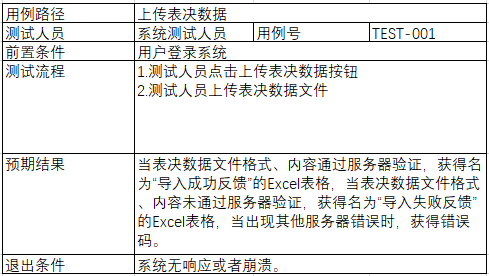
\includegraphics[height=5cm]{test1.png}
    \caption{测试用例表}
    \label{fig:test1}
  \end{figure}

  表~\ref{fig:test2}是我们进行功能性测试的结果。严重错误是指用户操作完系统无响应,系统发生了崩溃;而普通错误主要指在人机交互中的出错;而小错误则是一些显示上的字段错误或
  者页面编排上的小错误。在每次测试迭代过程中,我们都按照上一轮测试的结果不断进行
  修正,不断优化系统。

  \begin{table}[h!]
    \begin{center}
      \caption{系统功能性测试结果}
      \label{fig:test2}
      \begin{tabular}{ c c c c }
        \hline
        \textbf{测试轮数} & 1 & 2 & 3 \\
        \hline
        \textbf{小错误} & 28 & 5 & 0 \\
        \textbf{普通错误} & 20 & 2 & 0 \\
        \textbf{严重错误} & 5 & 1 & 0 \\
        \hline
      \end{tabular}
    \end{center}
  \end{table}

\section{系统性能测试}
在满足功能需求的前提下,我们需要保证系统的性能需求。本节性能测试将主要介绍三个测试,一是前端组件更新性能测试,二是 Mongo 写入性能测试,三是集群 Kafka 订阅发布性能测试。

\subsection{前端组件更新性能测试}
前端测试通过使用 immutable.js 写出测试页面,测试页面包含一个 table,通过脚本生成数据,更新数据并计算平均消耗时间,测试页面如图~\ref{fig:test3}。

\begin{figure}[!htp]
    \centering
    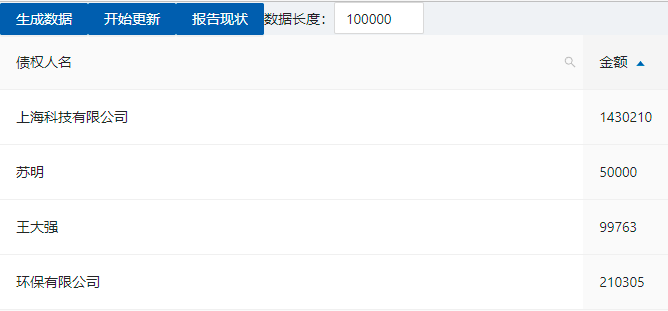
\includegraphics[height=6cm]{test3.png}
    \caption{前端测试页面}
    \label{fig:test3}
  \end{figure}

  为了测试前端在使用了 immutable.js 后,在 10000 条数据的情况下平均每条数据的更新所需时间,在测试页面输入数据长度为 10000,点击生成数据并点击开始更新,等待一段时间后点击报告现状,得到平均更新所需时间如如图~\ref{fig:test4},在表格 10000 条数据的情况下,平均更新每条信息所花费的时间为 18.73 ms,可以满足需求。

  \begin{figure}[!htp]
    \centering
    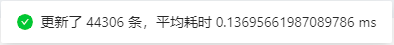
\includegraphics[height=2cm]{test4.png}
    \caption{前端测试结果}
    \label{fig:test4}
  \end{figure}

  \subsection{Mongo 写入性能测试}
  本文使用 Jmeter 测试工具进行了性能测试,测试了 Mongo 集群的写入性能。创建一个测试接口,此测试接口仅含有一次写入 Mongo 操作,通过 Jmeter 测试工具提升并发量,查看平均响应时间和 P95 响应时间,表~\ref{fig:test5}是我们进行测试的结果。根据性能测试的结果,可以推算出 Mongo 仅支持 700+ QPS,在高并发系统中明显为性能瓶颈。
  \begin{table}[h!]
    \begin{center}
      \caption{系统功能性测试结果}
      \label{fig:test5}
      \begin{tabular}{ c c c c }
        \hline
        \textbf{并发量} & \textbf{平均响应时间(ms)
        } & \textbf{P95值(ms)
        } & \textbf{P95平均值(ms)
        } \\
        \hline
        50 & 105 & 157 & 102 \\
        100 & 116 & 194 & 112 \\
        200 & 165 & 300 & 157 \\
        300 & 264 & 418 & 255 \\
        400 & 295 & 510 & 279 \\
        500 & 724 & 1007 & 702 \\
        600 & 864 & 1264 & 840 \\
        700 & 971 & 1559 & 937 \\
        800 & 1032 & 1584 & 997 \\
        900 & 1215 & 1864 & 1171 \\
        \hline
      \end{tabular}
    \end{center}
  \end{table}

  \subsection{Kafka 订阅发布性能测试}
  本视频表决会议系统作为高并发系统,可能存在短时间内请求过多使服务器服务宕机的情况,可能出现高并发情况的功能有实时表决和实时聊天,如果在短时间内大量债权人同时投票则实时表决会在短时间内出现大量请求,实时聊天同理,由于并发都是针对于实时性的功能,性能瓶颈需要考虑实时 WebScoket 端性能和 Mongo 的写入性能,而前面测试得到 Mongo 的写入性能无法满足系统的要求,为系统的性能瓶颈,仅仅通过增加服务实例的方式无法解决请求过多的情况,因此在 WebSocket端还需要进行流量削峰,本系统使用消息中间件 Kafka 达到流量削峰的目的,本节将测试 Kafka 订阅发布的性能,来确认 Kafka 的性能是否满足要求,是否会成为系统的性能瓶颈。

  测试在 100 个分区,1 个订阅的情况下测试订阅发布的延迟,结果表~\ref{fig:test6},所示。当ack=1,消息被追加到leader副本所在分区后再确认,当ack=all,在所有的ISR(同步副本)都接收到消息时才确认,在这两种情况下,平均响应时间为 4+ ms,能够满足系统需求。

  通过对 Mongo 写入性能的测试和对 Kafka 订阅发布性能的测试结果进行对比后发现,可以确定本系统性能瓶颈为 Mongo 写入性能,因此后续出现性能瓶颈时需要考虑对系统 Mongo 的写入性能进行优化。

  \begin{table}[h!]
    \begin{center}
      \caption{系统功能性测试结果}
      \label{fig:test6}
      \begin{tabular}{ c c c c }
        \hline
        \textbf{类型} & \textbf{平均响应时间(ms)
        } & \textbf{P90值(ms)
        } & \textbf{P99值(ms)
        } \\
        \hline
        Kafka-ack-1 & 4.26 & 5.39 & 6.94 \\
        Kafka-ack-all & 4.22 & 5.19 & 10.43 \\
        \hline
      \end{tabular}
    \end{center}
  \end{table}